
\chapter{Вводная электронная схема}

\section{Где купить комплектующие?}

В Новой Зеландии есть некоторое количество отличных поставщиков компонентов с
разумными ценами, включающих \url{www.surplustronics.co.nz}, и
\url{www.activecomponents.com}. Зарубежные поставщики, которых я использую,
включают \url{www.digikey.co.nz}, \url{www.sparkfun.com}, \url{ebay.com}
и \url{aliexpress.com}

\bigskip
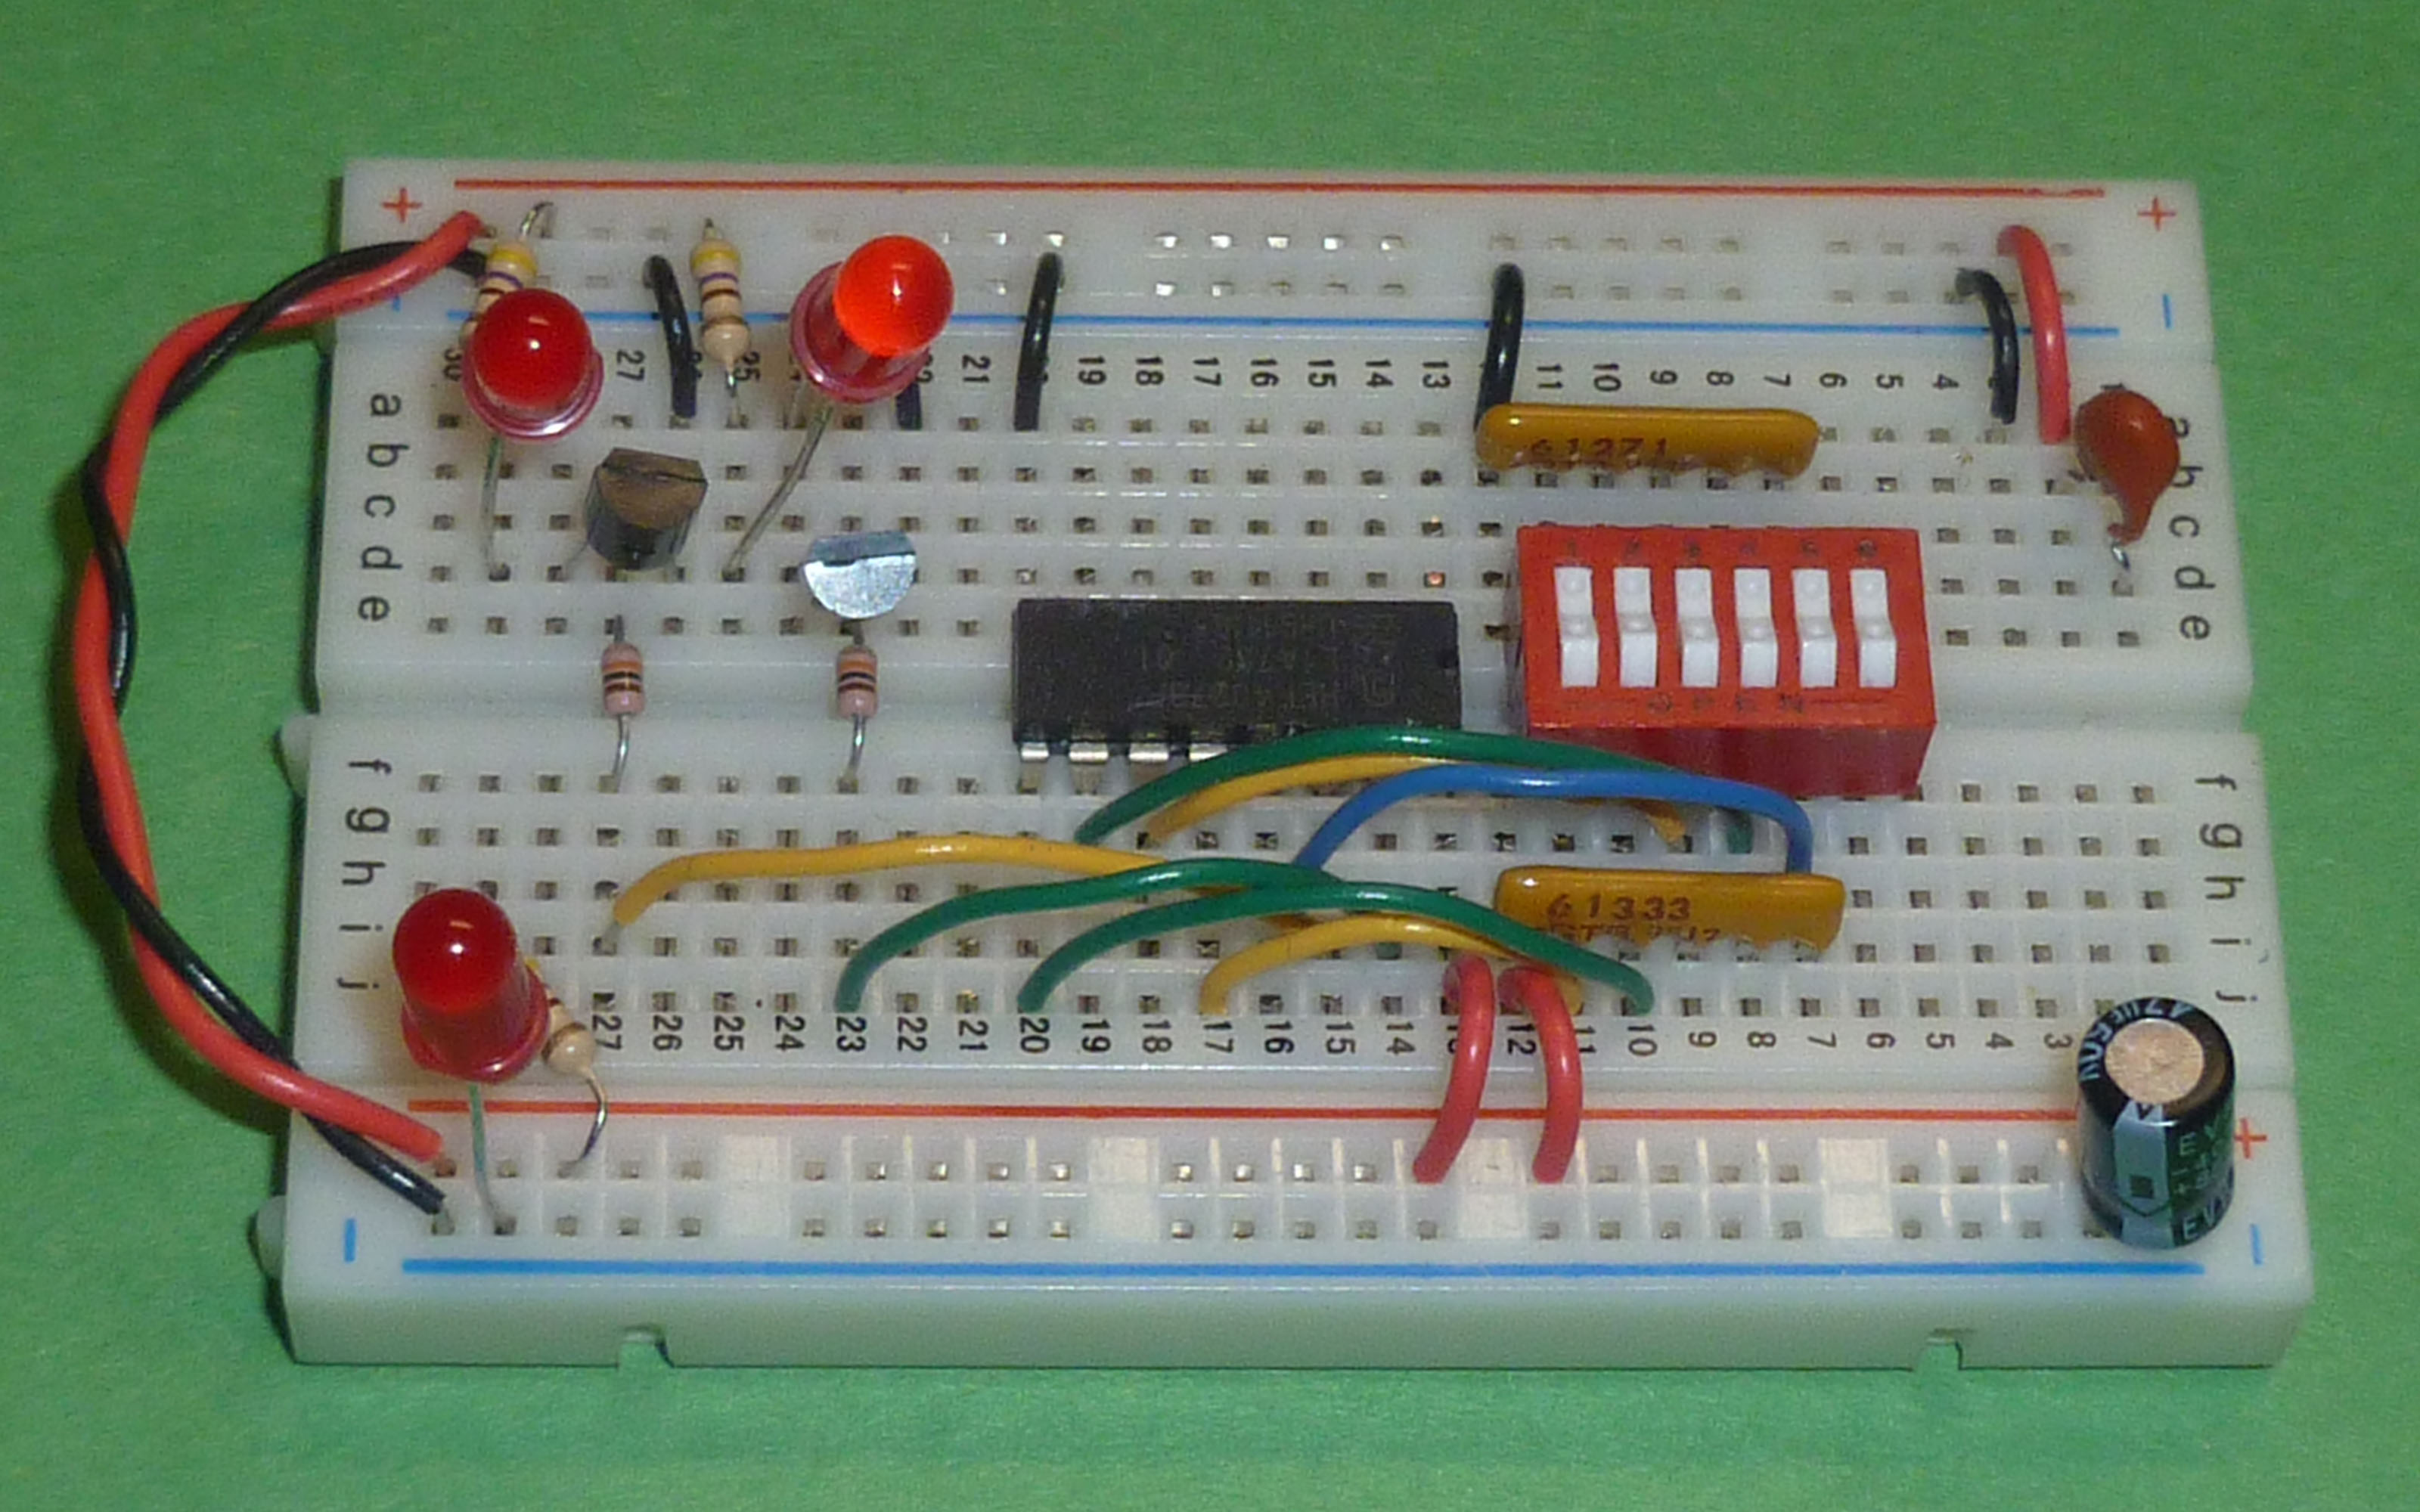
\includegraphics[width=0.8\textwidth]{bcollis/breadboard2.jpg}

\term{Breadboard} ([б]еспаечная [м]акетная [п]лата , БМП, ``вафля'')\ ---
пластмассовый блок с отверстиями и металлическими полоск\'{о}выми зажимами,
создающими соединения между \term{элементами схемы}. Отверстия расположены так,
что \term{компоненты} и отрезки провода могут быть соединены вместе формируя
схему, без использования паяльника. Верхние и нижние ряды, как правило,
используются для шин питания, красный сверху для плюса, и внизу черный/синий для
минуса (общий провод). На длинных вафлях \term{шины питания} поделены на
отдельные сегменты, и требуют соединения короткими перемычками.

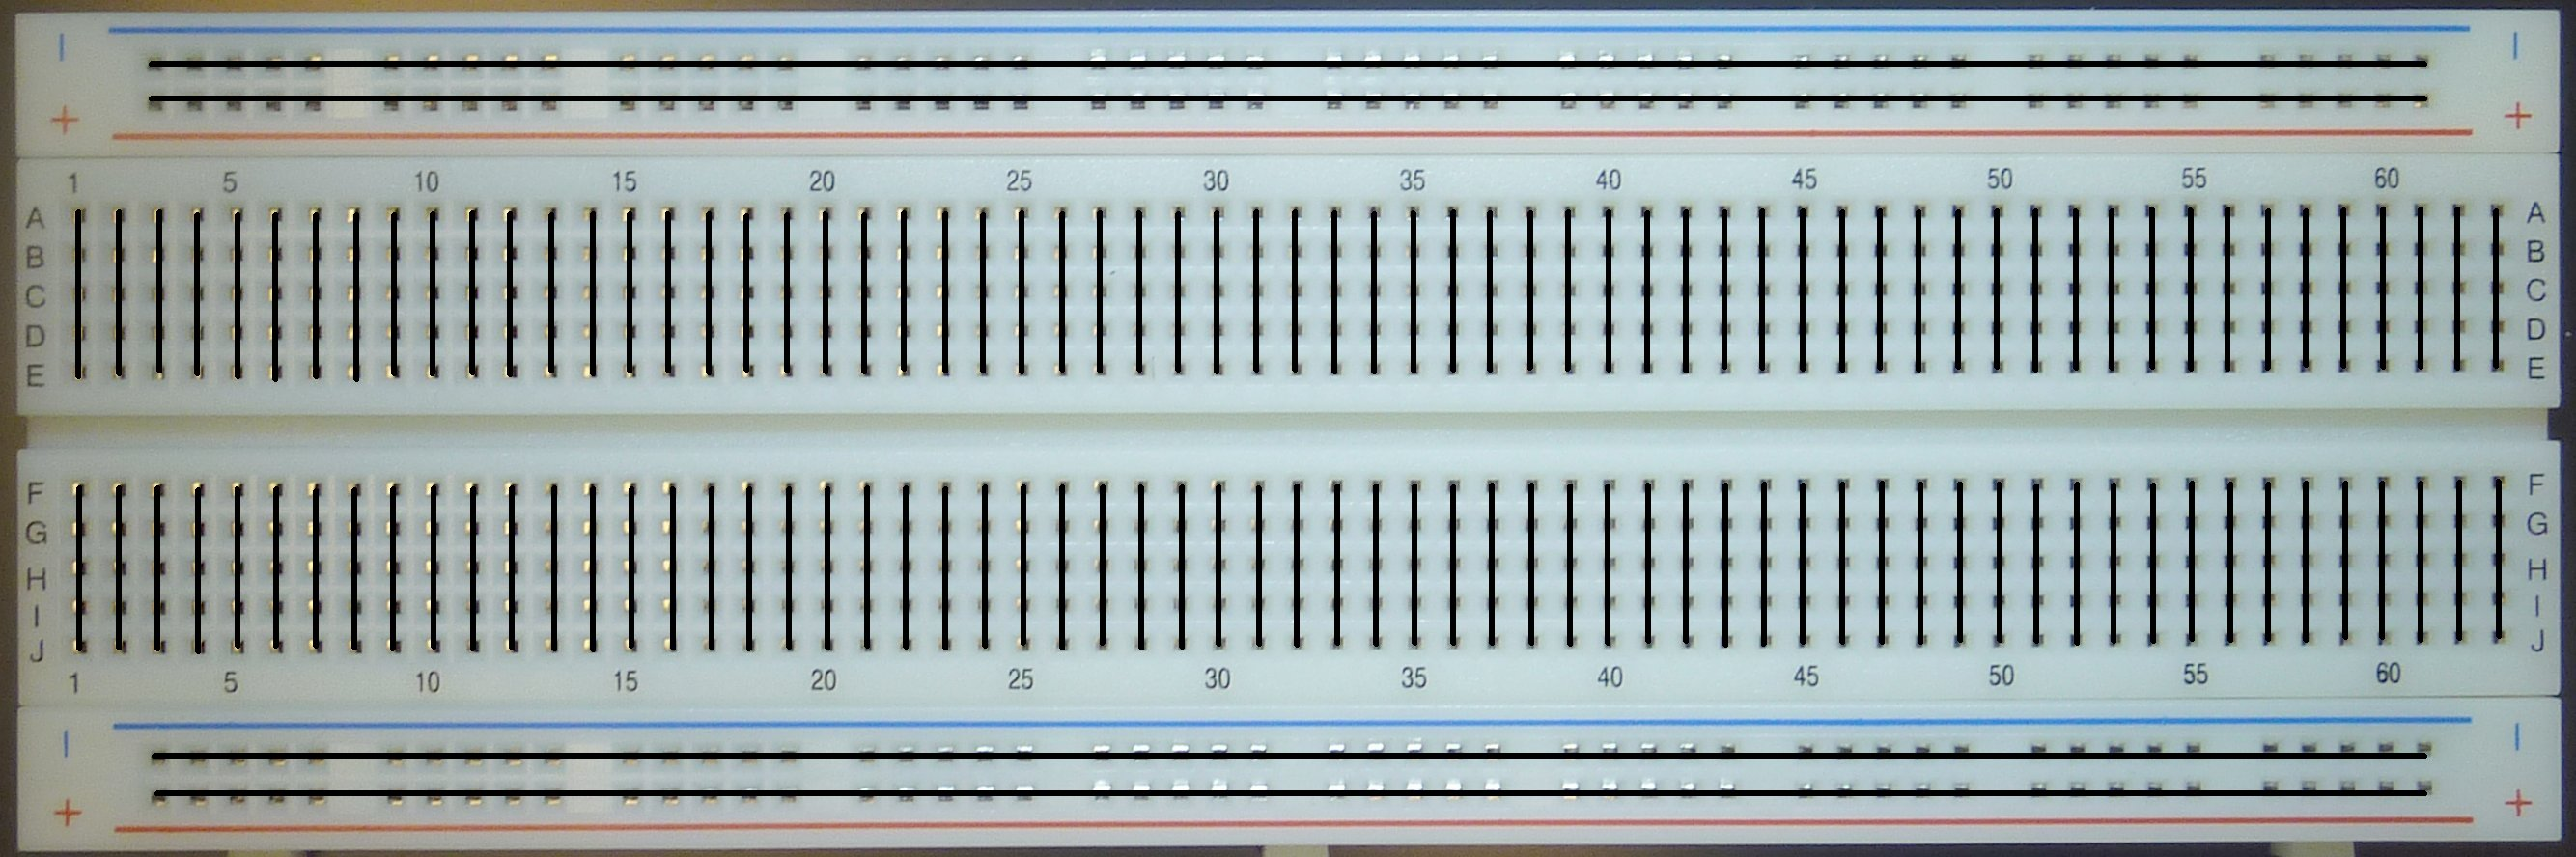
\includegraphics[width=0.8\textwidth]{bcollis/BreadboardConnections.jpg}

\bigskip

Эта схема \ref{ch21sch}\ может быть собрана вот так \ref{ch21lay}, обратите
внимание, что \term{светодиод} должен находиться в правильном положении. Если у
вас есть светодиод и \term{резистор}, соединенные в \term{замкнутый контур},
светодиод должен загореться.

\bigskip
Принципиальная схема \label{ch21sch}

\bigskip
Компоновка \label{ch21lay}

\bigskip
Светодиоду требуется \emph{для включения} около 2\,В\note{[В]ольт}, батарея на
9\,В, так что с напряжением все нормально.
\emph{Но если вы подключите светодиод напрямую к батарее, 
он сгорит! Для светодиодов главный рабочий параметр\ --- \term{допустимый
рабочий ток}, обычно он не превышает 10..20\,mA\note{1\,[м]иллиАмпер =
0.001\,[А]мпер}}. Так что 1\,k\note{1\,[К]илоОм = 1000\,Ом}\ резистор
используется для ограничения тока через светодиод.

\bigskip
Если вы отключите любой провод в схеме, она перестает работать, схема должна
быть завершенной, чтобы электроны могли течь.

\section{Использование мультиметра}

Возьмите мультиметр\ref{mmetr}\ и измерьте напряжение на резисторе, близко ли
оно к 7\,В ? Также измерьте ток через диод, не превышает ли он допустимый ?

\begin{framed}
\emph{Напряжение} измеряется \term{в [В]\'{о}льтах} подключением
\term{измерительного прибора} (мультиметра) \emph{параллельно}\ элементу, при этом нужно
\begin{itemize}
\item
\term{режим измерения} включить на
\term{режим измерения постоянного напряжение} $V-$/DCV (или переменного,
обозначается как $V\sim$/ACV) а
  \item \term{диапазон
измерения} \emph{выставить на максимальное значение напряжения}
\item 
Последовательно уменьшая диапазон измерения, найдите диапазон, в котором
мультиметр показывает наибольшее количество знаков после запятой. 
\end{itemize}
\end{framed}

Если диапазон
слишком большой, прибор покажет значение в районе 0, а если слишком низкий\ ---
выведет [1]. Обычно работают в диапазоне, соответствующем максимальому
напряжению питания (в нашем случае 20\,V\note{[V]olt = [В]ольт}), иногда для
слабых напряжений переключаясь на одну..две ступени ниже. Но\ ---
\emph{возможны случаи\note{в \emph{любых схемах} содержащих
\term{индуктивности}: катушки пр\'{о}вода, трансформаторы, электродвигатели,
динамики и т.п.} когда напряжение в части схемы на порядки (в десятки..тысячи
раз) превосходит напряжение питания}.

\begin{framed}
\emph{Ток} измеряется \term{в [А]мп\'{е}рах} подключением \term{измерительного
прибора} (мультиметра) \emph{последовательно}\ с элементом \term{в разрыв цепи}, при этом
нужно
\begin{itemize}
\item
\term{режим измерения} включить на
\term{режим измерения постоянного тока} $A-$/DCA (или переменного, обозначается
как $A\sim$/ACA) а
  \item \term{диапазон
измерения} \emph{выставить на максимальное значение тока}
\item 
Последовательно уменьшая диапазон измерения, найдите диапазон, в котором
мультиметр показывает наибольшее количество знаков после запятой. 
\end{itemize}
\end{framed}

Обратите внимание, что напряжение измеряется \term{вольтметром} на полностью
собранной схеме, а для измерения тока нужно изменять схему, включая в нее
\term{амперметр}. Если измерения тока нужно проводить на готовом устройстве,
иногда ставят 2хконтактный \term{джампер} (как на материнских платах
компьютеров): при измерении амперметр подключают к его контактам, а потом
джампер замыкают специальной съемной проводящей перемычкой. Этом прием вы можете
использовать в своих устройствах для регулярного измерения \term{тока
потребления}, и расчета \term{потребляемой мощности}:

\begin{equation}
W_{\mbox{потребляемая}}\mbox{[Ватт]} = 
U_{\mbox{питания}}\mbox{[Вольт]} 
\times
I_{\mbox{устройства/элемента}}\mbox{[Ампер]}
\end{equation}

\begin{framed}
Переключив мультиметр в \term{режим прозвонки (т\'{е}стера)}, можно проверить
\begin{itemize} 
\item наличие
электрического соединения между двумя точками \emph{обязательно отключенной от
источника питания} схемы,
\item исправность диода или светодиода,
\item исправность конденсатора большой \term{емкости} и
\item любые другие случаи когда нужно определить что две точки электрически
соединены между собой, постоянно или временно.
\end{itemize}
\end{framed}

Если между \term{щщуп}ами мультиметра в режиме прозвонки\note{= тестера}\
\term{сопротивление} протекающему току не превышает 1\,КилоОм\note{см.
паспорт на прибор}, раздается звуковой сигнал.

Если щщупы подключить к исправному \emph{разряженному} конденсатору большой
емкости (``электролиту''), раздастся короткий целчок или даже ``пик''.

Тестером также можно определить тип и \term{цокол\'{е}вку\note{``раскопытку''}}
транзистора; как это сделать описано в \ref{vt}.

\emph{Диоды} проверяются двумя подключениями \emph{в разной полярности}\ --- при
\emph{красном щщупе} на \term{аноде (+)} диода (в \term{прямой полярности
включения}) диод проводит ток, а в \term{обратной полярности} нет (красный щщуп
на \term{катоде (-)}).

Проверьте \emph{светодиод}: отключите его из схемы, и проверьте как диод.
Если светодиод исправен, в \emph{прямой полярности} светодиод будет \emph{очень
слабо светиться}.

\section{2.2 Определение сопротивления резистора по цветовому коду 16}

.

\section{2.3 Светодиоды 17}

.

\section{2,4 Некоторые технические характеристики светодиода 17}

.

\section{2.5 Задание на исследование светодиода 17}

.

\section{2.6 Добавление выключателя  в схему 18}

.

\section{2.7 Задание на установку выключателя 18}

.

\section{2,8 Важные понятия схемы 19}

.

\section{2.9 Изменение величины сопротивления 19}

.

\section{2.10 Добавление транзистора в схему 20}

.

\section{2.11 Чтение схем 21}

.

\section{2.12 Входная цепь\ --- LDR 22}

.

\section{2.13 Рабочая схема датчика темноты 23}

.

\section{2,14 Защитные цепи - использование диода 24}

.

\section{2.15 Задача исследования диода 24}

.

\section{2.13 Финальная схема датчика темноты 23}

.

